\chapter{Oracle Aplication Express}

\section{Tahapan Pembuatan Aplikasi Yang Berjudul Academic Sederhana}
Pada Langkah pertama yang harus dilakukan untuk membuat sebuah aplikasi pada Apex Oracle adalah membuka website https://apex.oracle.com dan masuk untuk login, setelah login Berikut di bawah ini adalah langkah - langkah pembuatan Aplikasi pada Oracle APEX :

\begin{enumerate}
\item[1]Yang pertama Jika sudah login maka akan Masuk Ke tampilan Seperti ini, lalu klik create untuk memasukan database yg sudah kita buat di Excel.

\begin{figure}[!htbp]
    \begin{center}
    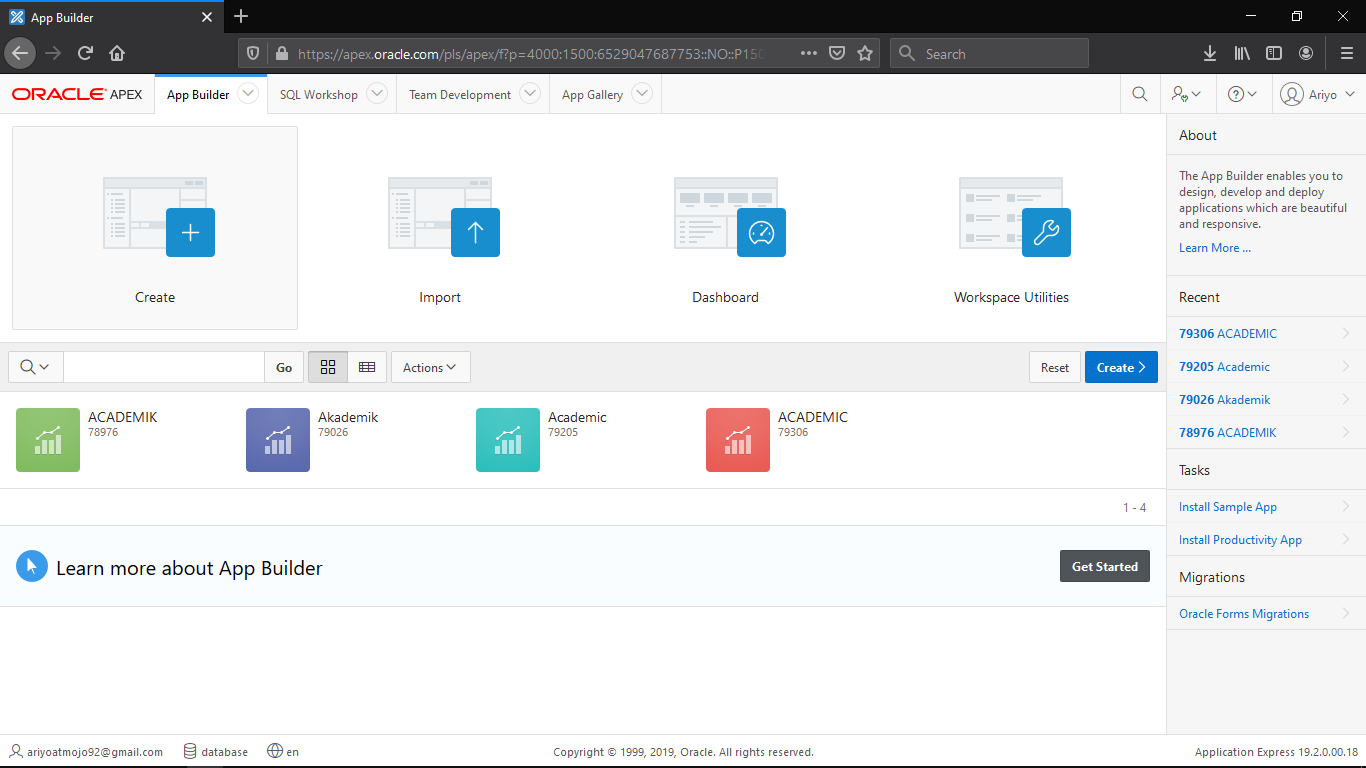
\includegraphics[scale=0.2]{figures/1.png}
    \caption{\textit{}}
    \end{center}   
    \end{figure}
    
\begin{figure}[!htbp]
\item[2]Setelah itu klik From a file.

    \begin{center}
    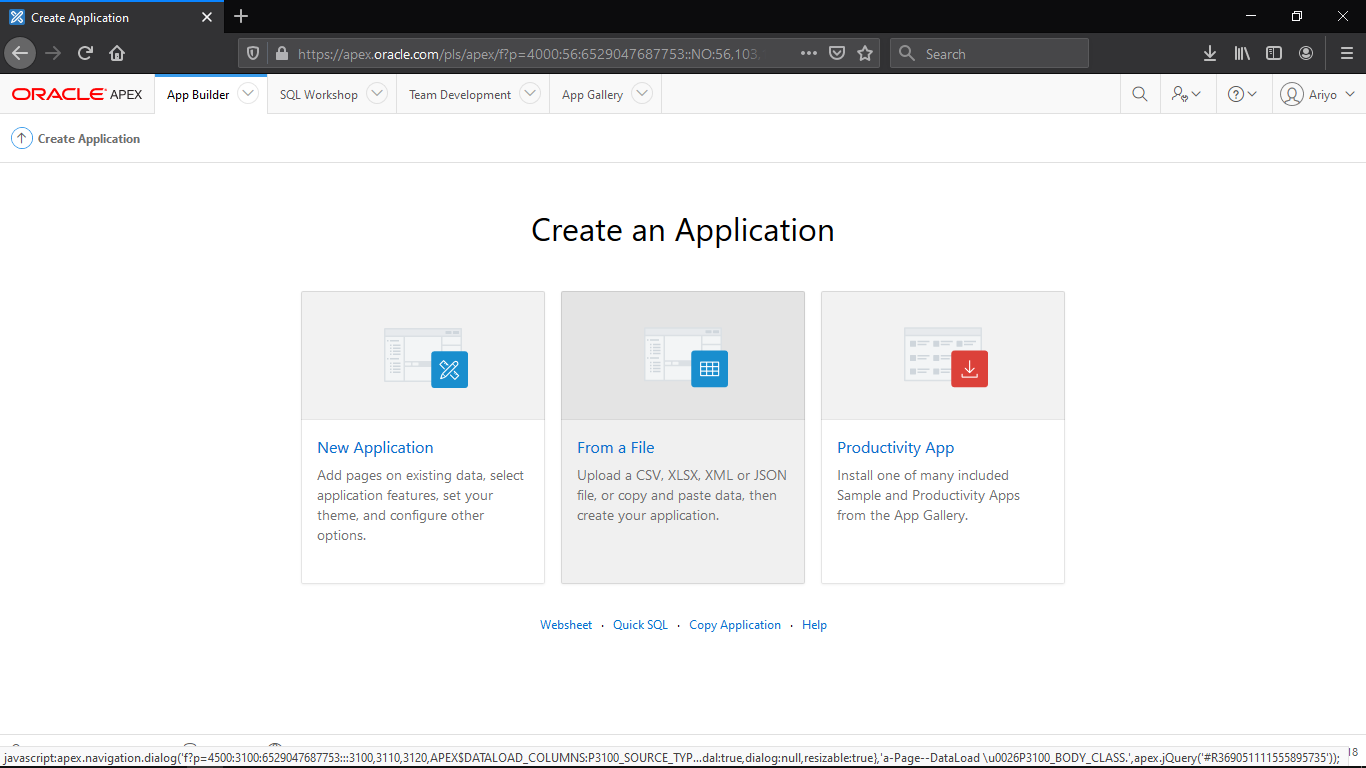
\includegraphics[scale=0.2]{figures/2.png}
    \caption{\textit{}}
    \end{center}


\item[3]Lalu klik Choose File dan pilih data yg ingin dimasukkan dari excel yg sudah dibuat, setelah itu buat Tablenya seperti gambar dibawah ini.

    \begin{center}
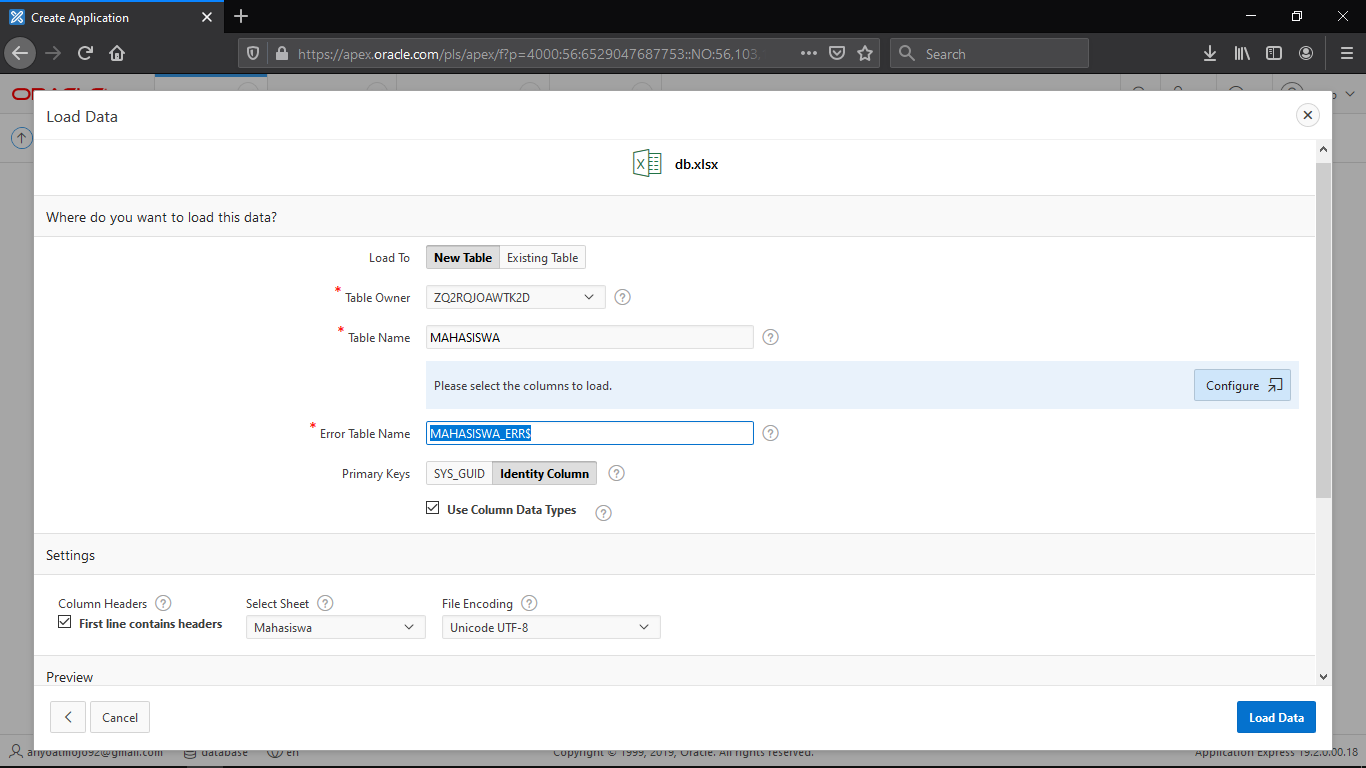
\includegraphics[scale=0.2]{figures/4.png}
    \caption{\textit{}}
        \end{center}
\label{gambar}
\end{figure}

\begin{figure}
\item[4]Dan tampilan dibawah ini adalah table yg sudah dibuat, dan nama tablenya adalah Mahasiswa.

    \begin{center}
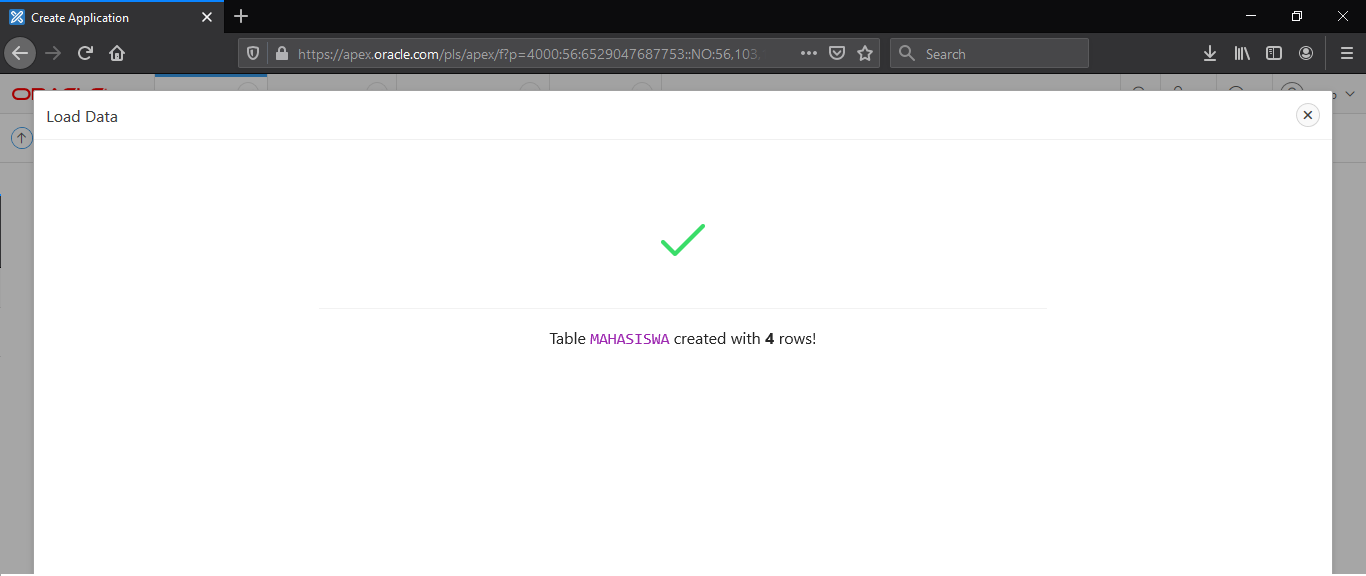
\includegraphics[scale=0.2]{figures/5.png}
    \caption{\textit{}}
        \end{center}
\label{gambar}
\end{figure}

\begin{figure}
\item[5]Setelah itu buat lagi sampai 5 Table dan nama tablenya adalah Dosen, Jadwal, Kuliah, Mahasiswa, Nilai, tampilannya seperti dibawah ini.

    \begin{center}
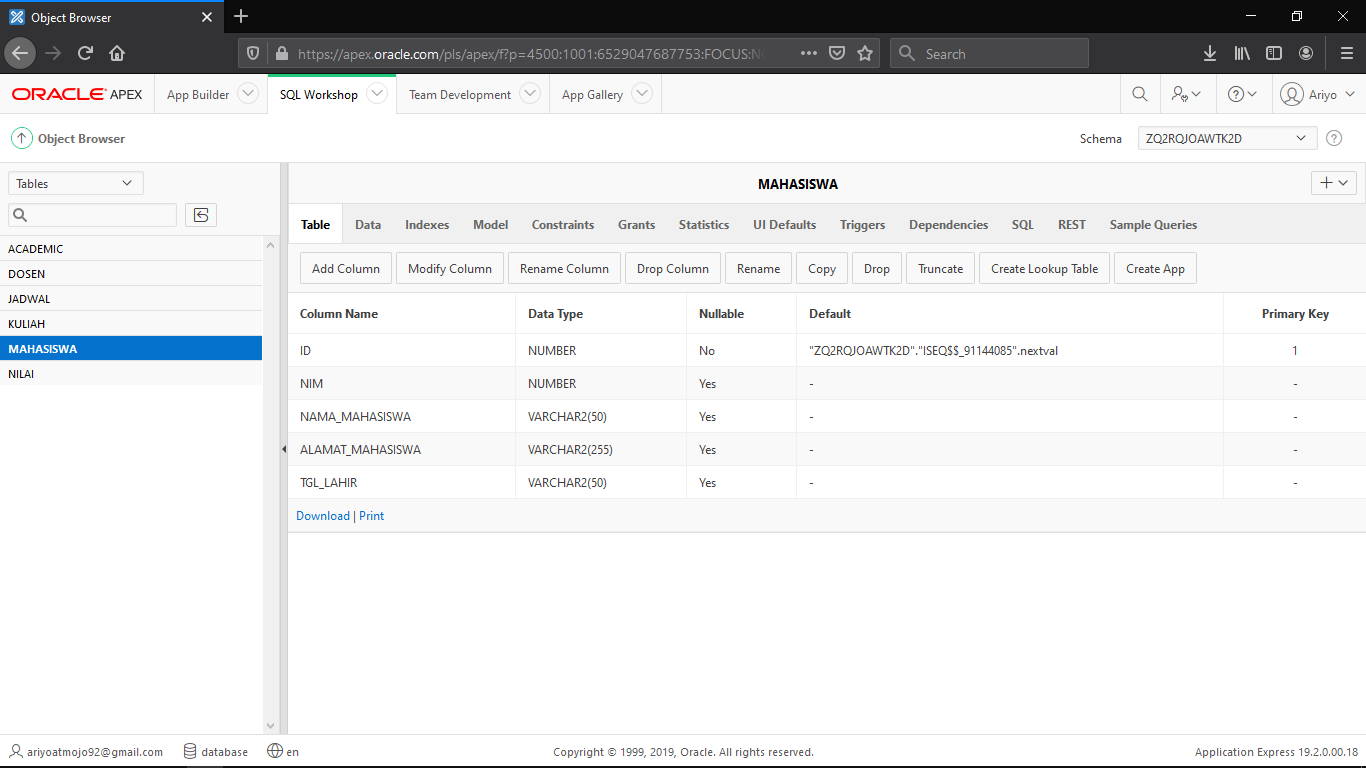
\includegraphics[scale=0.2]{figures/14.png}
    \caption{\textit{{}l}}
        \end{center}
\label{gambar}
\end{figure}

\begin{figure}
\item[6]Setelah itu didalam table ada sebuah ID dan harus kita hilangkan karena kita belum membuat primary keynya, apex secara otomatis menciptakan atribut baru sebagai primary key dengan nama ID, langkah - langkahnya adalah klik Drop Clumn dan rubah seperti gambar dibawah ini. 

    \begin{center}
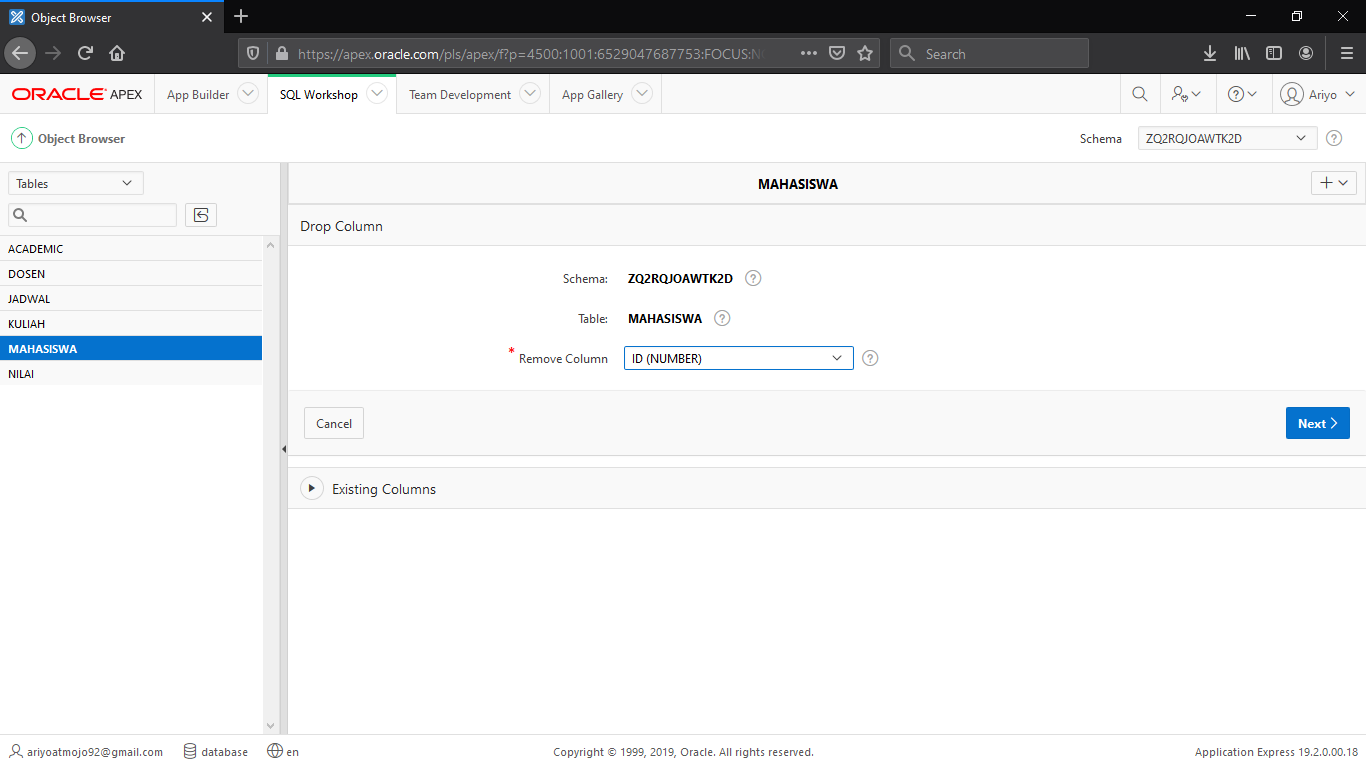
\includegraphics[scale=0.2]{figures/15.png}
    \caption{\textit{}}
        \end{center}
\label{gambar}
\end{figure}

\begin{figure}
\item[7]Dan juga di Table Nilai harus di hapus, sampai ke 5 table itu seperti sisanya adalaha nilai kuliah, jadwal, dosen juga harus di hapus.

    \begin{center}
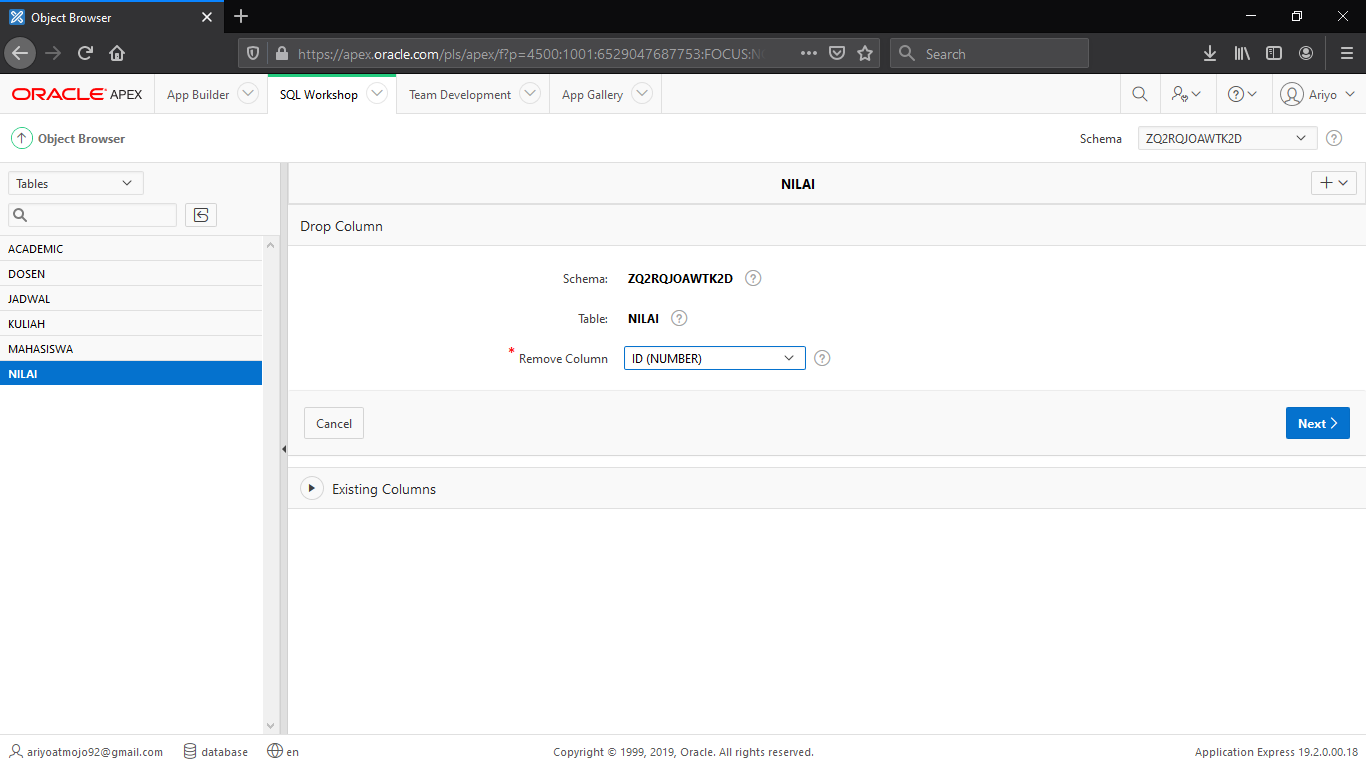
\includegraphics[scale=0.2]{figures/16.png}
    \caption{\textit{}}
        \end{center}
\label{gambar}
\end{figure}

\begin{figure}
\item[8]Jika sudah semua, klik Constraints lalu klik Create.

    \begin{center}
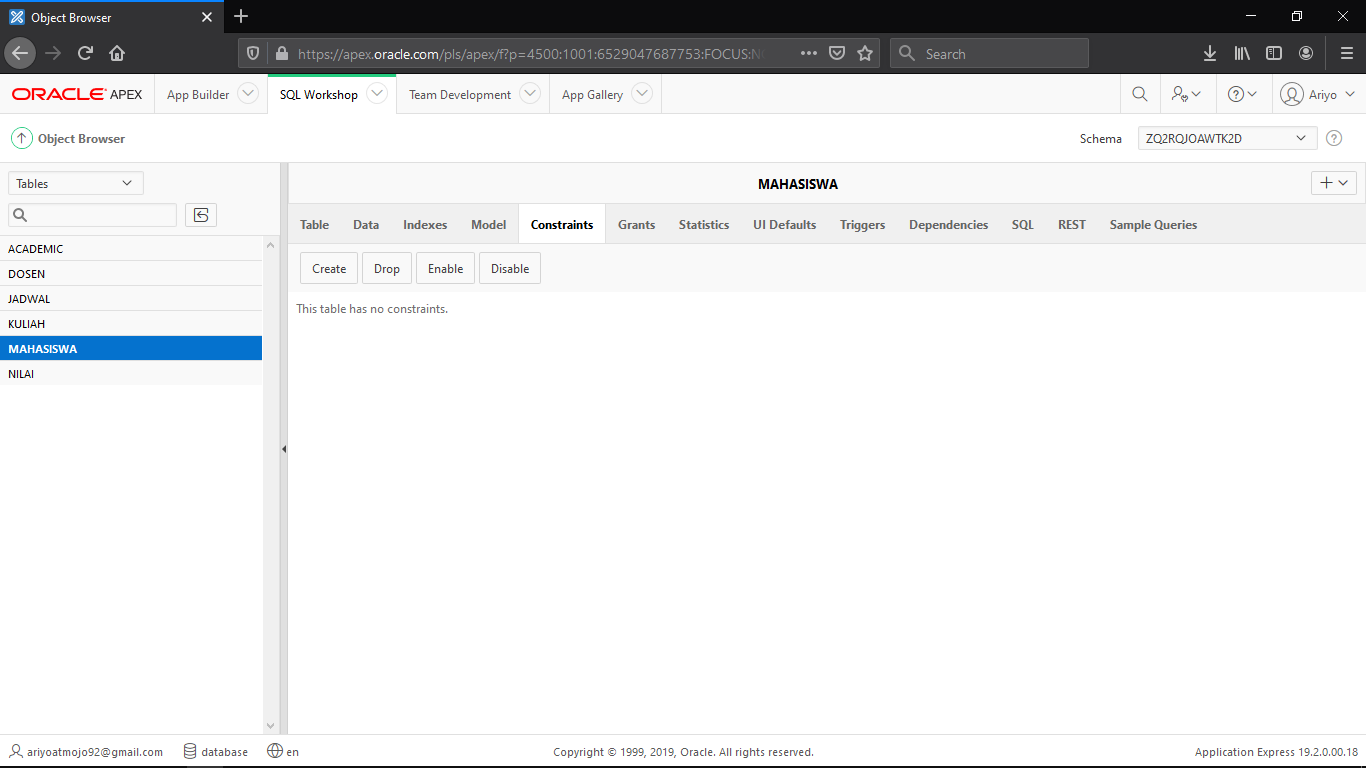
\includegraphics[scale=0.2]{figures/20.png}
    \caption{\textit{}}
        \end{center}
\label{gambar}
\end{figure}

\begin{figure}
\item[9]Lalu dalam table mahasiswa kita buat NIM dijadikan primary key seperti tampilan dibawah ini.

    \begin{center}
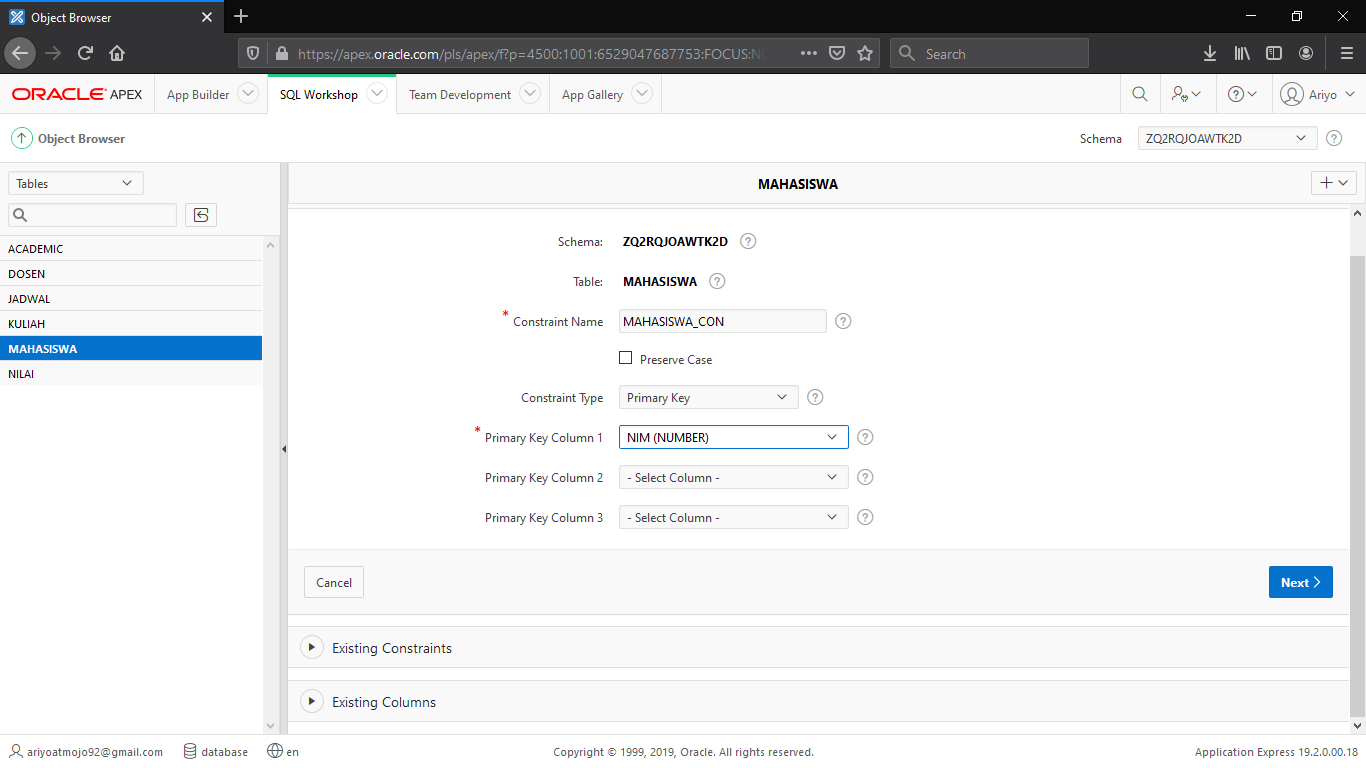
\includegraphics[scale=0.2]{figures/21.png}
    \caption{\textit{}}
        \end{center}
\label{gambar}
\end{figure}

\begin{figure}
\item[10]Dan hasilnya seperti ini.

    \begin{center}
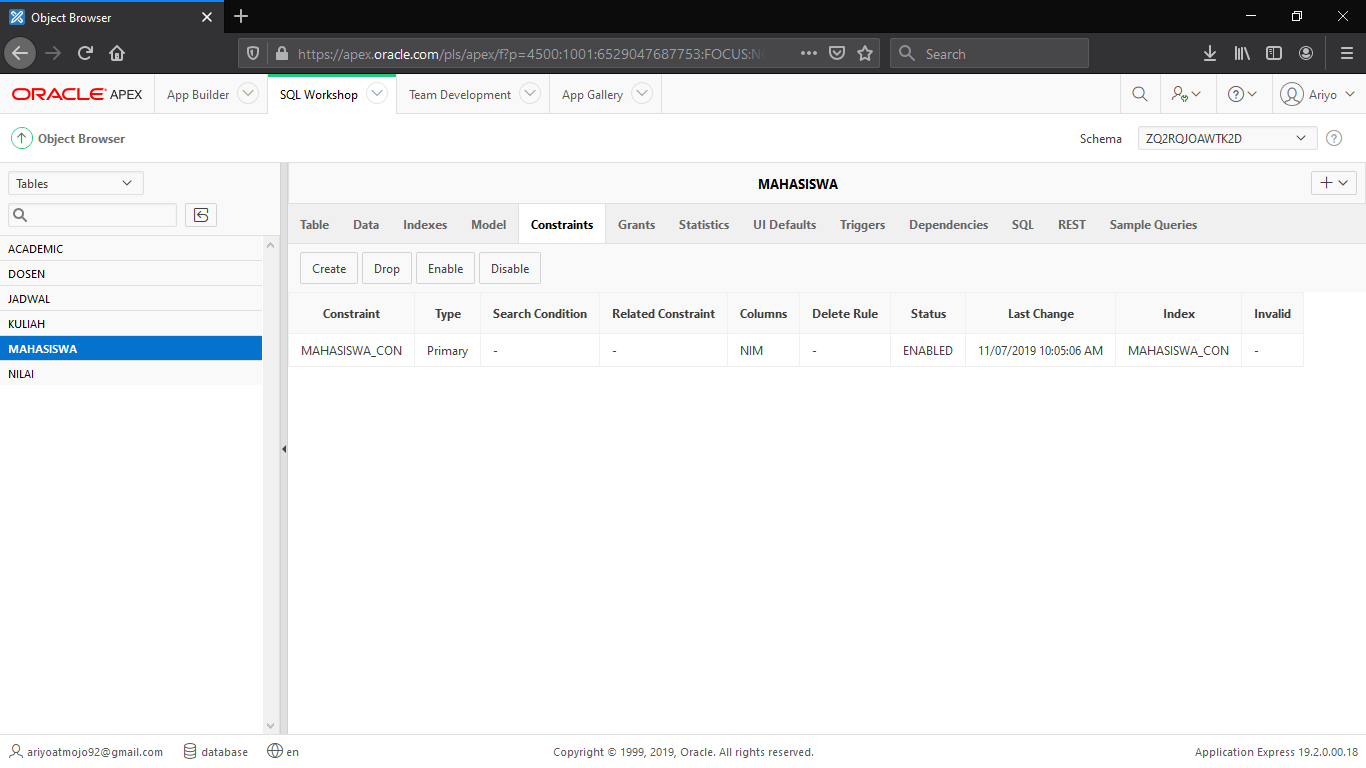
\includegraphics[scale=0.2]{figures/22.png}
    \caption{\textit{}}
        \end{center}
\label{gambar}
\end{figure}

\begin{figure}
\item[11]Dan juga di table nilai buat NIM dan KODE jadikan Foreign Key seperti dibawah ini.
    \begin{center}
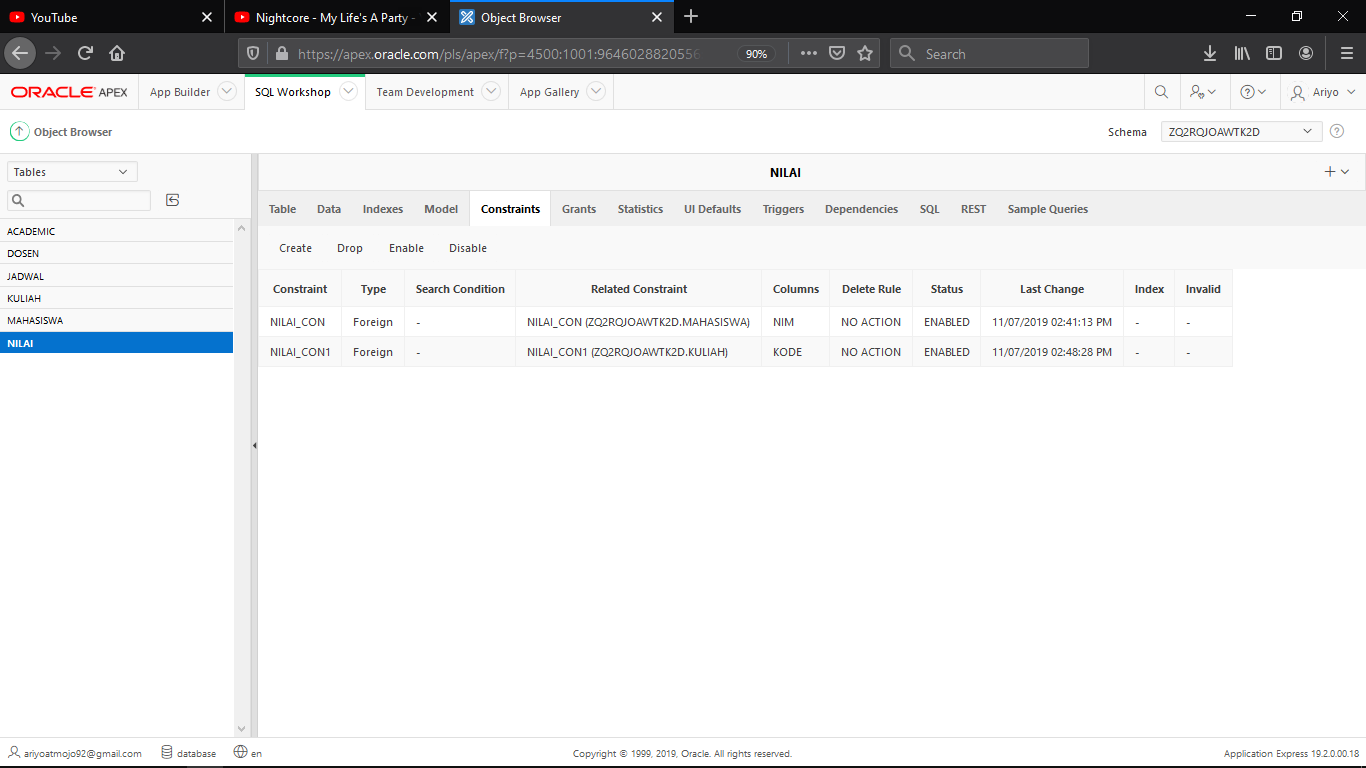
\includegraphics[scale=0.2]{figures/23.png}
    \caption{\textit{}}
        \end{center}
\label{gambar}
\end{figure}

\begin{figure}
\item[12]Lalu di dalam Table kuliah diberi juga KODE dijadikan Primary Key.

    \begin{center}
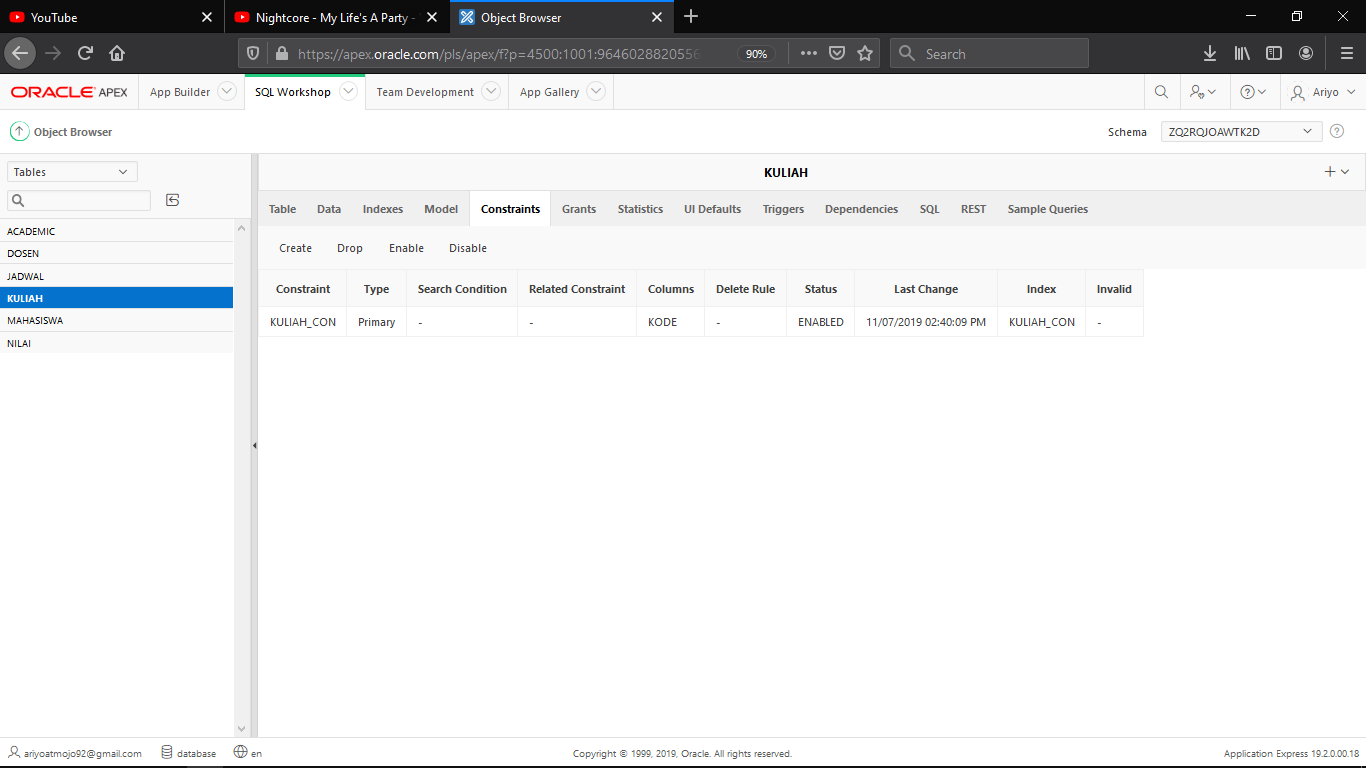
\includegraphics[scale=0.2]{figures/24.png}
    \caption{\textit{l}}
        \end{center}
\label{gambar}
\end{figure}

\begin{figure}
\item[13]Jika sudah masuk ke App builder lalu klik Create dan klik New Application.

    \begin{center}
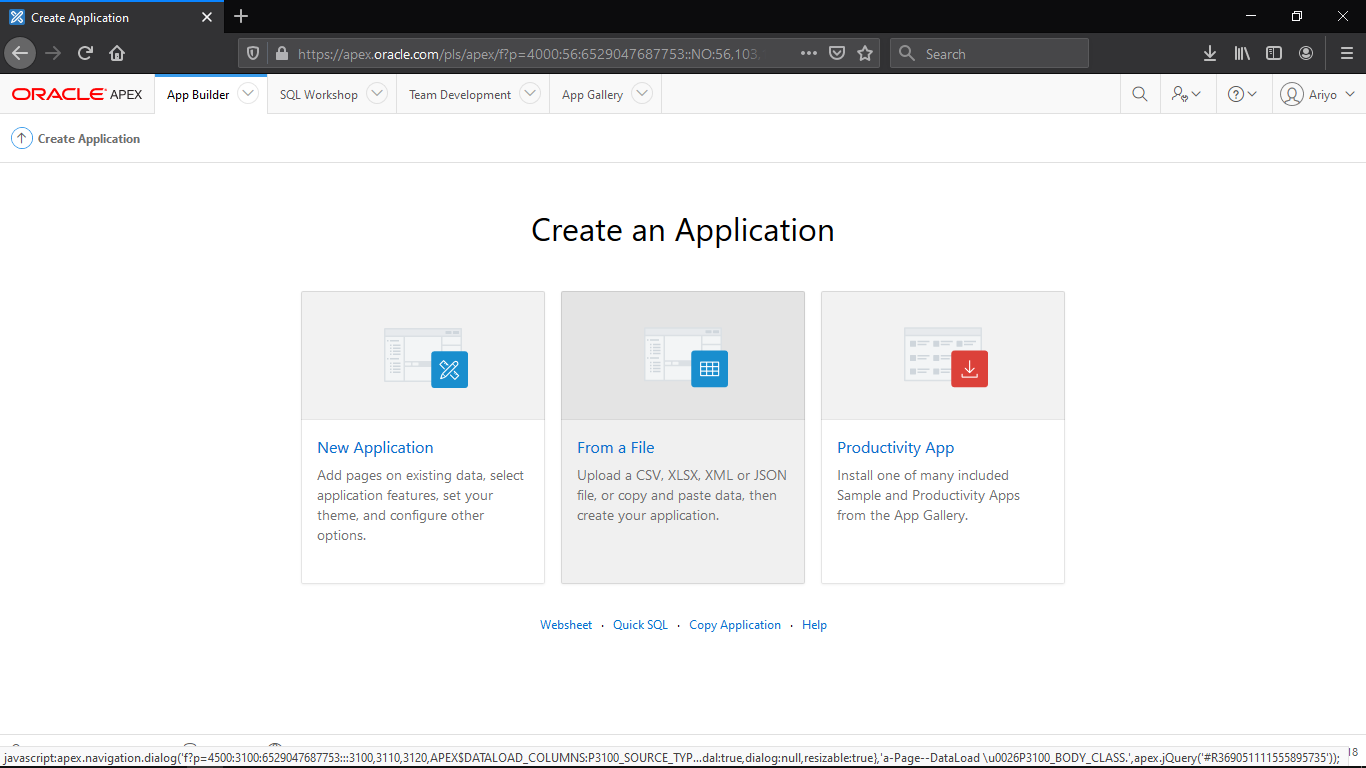
\includegraphics[scale=0.2]{figures/2.png}
    \caption{\textit{}}
        \end{center}
\label{gambar}
\end{figure}


\begin{figure}
\item[14]Setelah itu Klik Add Master Detail dan beri nama pagenya adalah Mahasiswa, dan nama table juga mahasiswa lalu ikutin seperti tampilan dibawah ini.

    \begin{center}
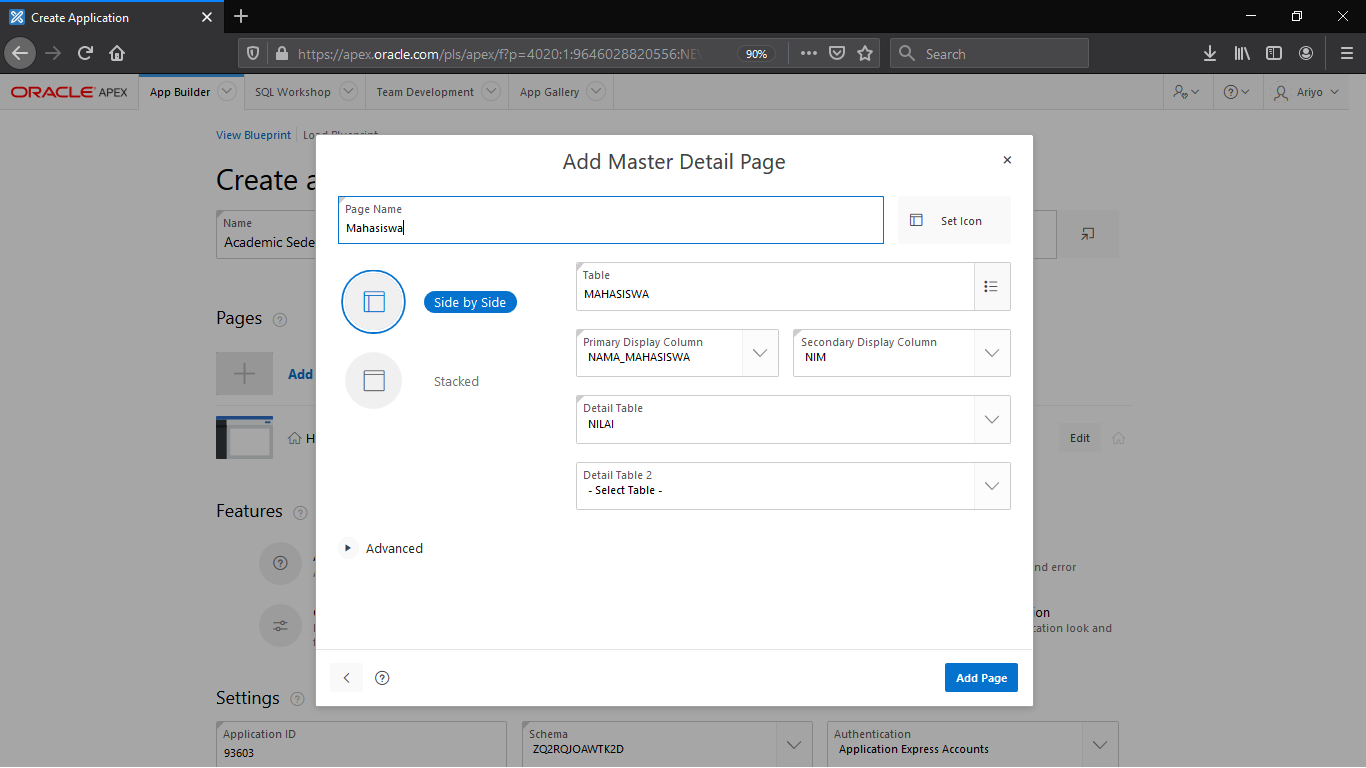
\includegraphics[scale=0.2]{figures/28.png}
    \caption{\textit{}}
        \end{center}
\label{gambar}
\end{figure}


\begin{figure}
\item[15]Dan lanjutkan juga buat tampilan Dosen seperti dibawah ini.

    \begin{center}
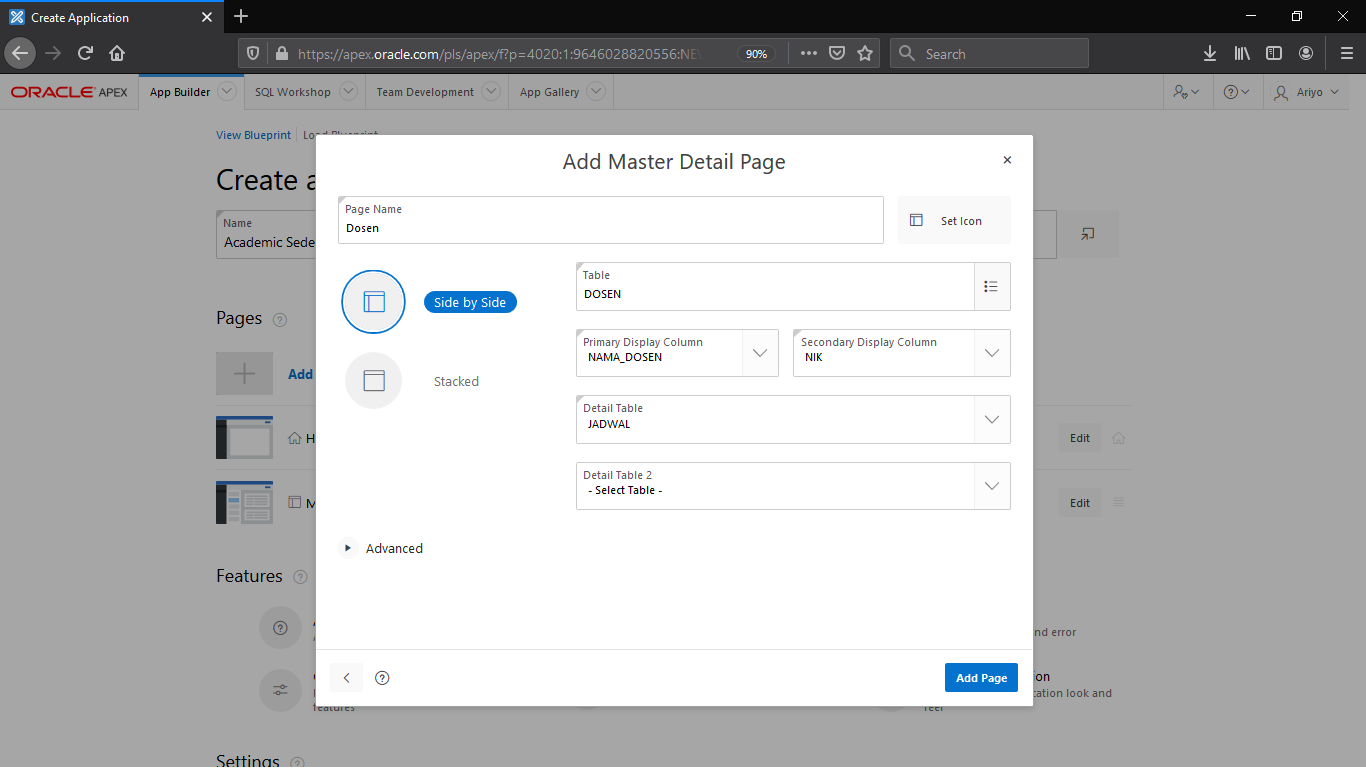
\includegraphics[scale=0.2]{figures/29.png}
    \caption{\textit{}}
        \end{center}
\label{gambar}
\end{figure}


\begin{figure}
\item[16]Jika Sudah buat Master Pagenya, setelah itu buat Interactive Reportnya di dalam Add Page dan ikutin seperti tampilan dibawah ini.

    \begin{center}
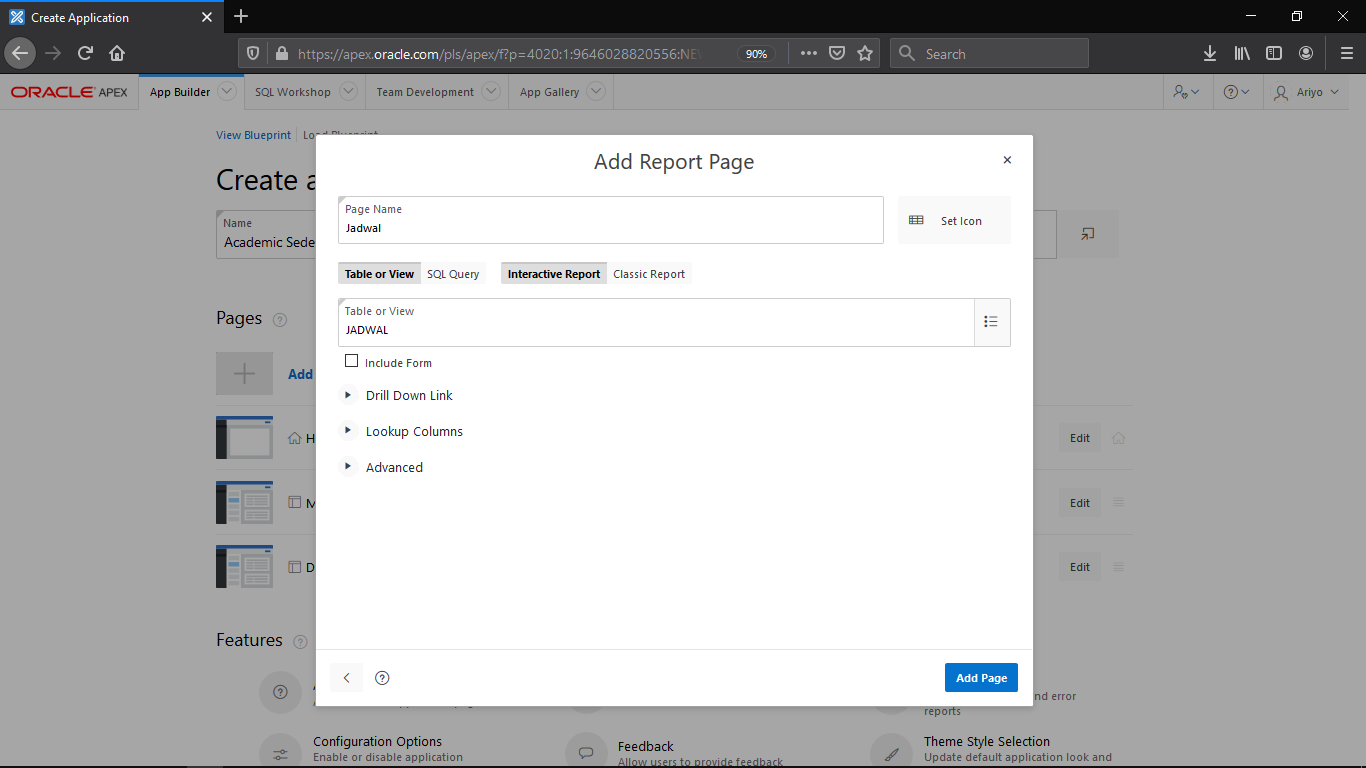
\includegraphics[scale=0.2]{figures/30.png}
    \caption{\textit{}}
        \end{center}
\label{gambar}
\end{figure}


\begin{figure}
\item[17]Dan tambah juga Interactive Reportnya di Nilai.

    \begin{center}
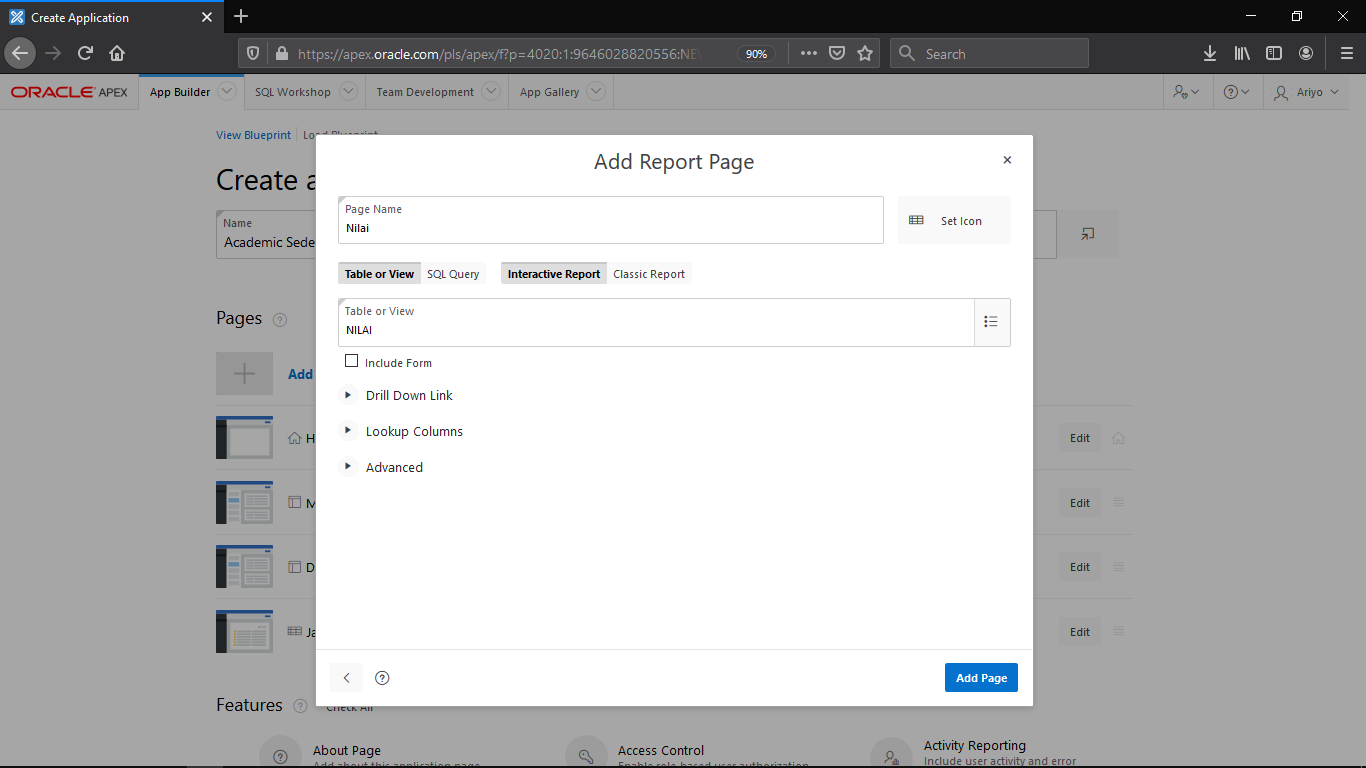
\includegraphics[scale=0.2]{figures/31.png}
    \caption{\textit{}}
        \end{center}
\label{gambar}
\end{figure}


\begin{figure}
\item[18]Setelah itu tambah lagi di Page Kuliah.

    \begin{center}
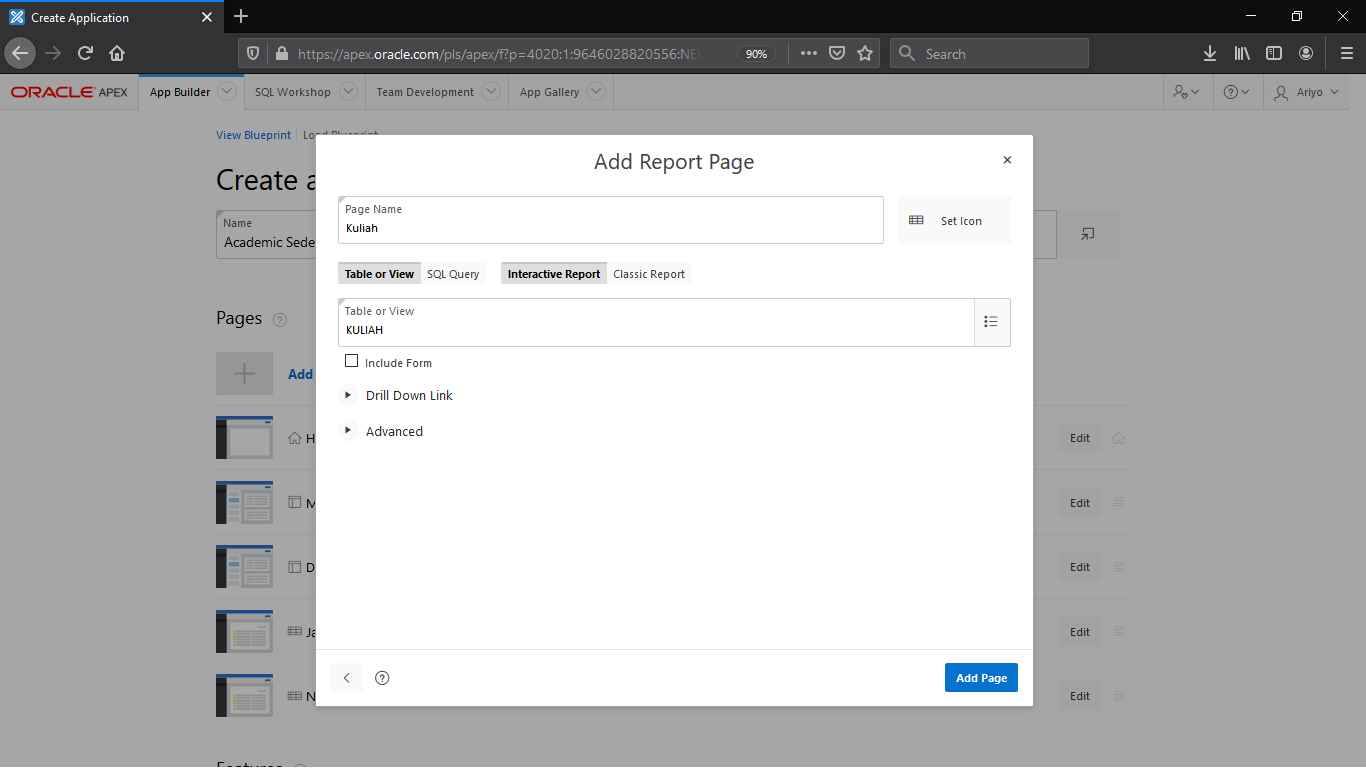
\includegraphics[scale=0.2]{figures/32.png}
    \caption{\textit{}}
        \end{center}
\label{gambar}
\end{figure}


\begin{figure}
\item[19]Jika sudah buat Dashboard di App Pagenya untuk Mahasiswa, dan ikuti tampilan seperti dibawah ini.

    \begin{center}
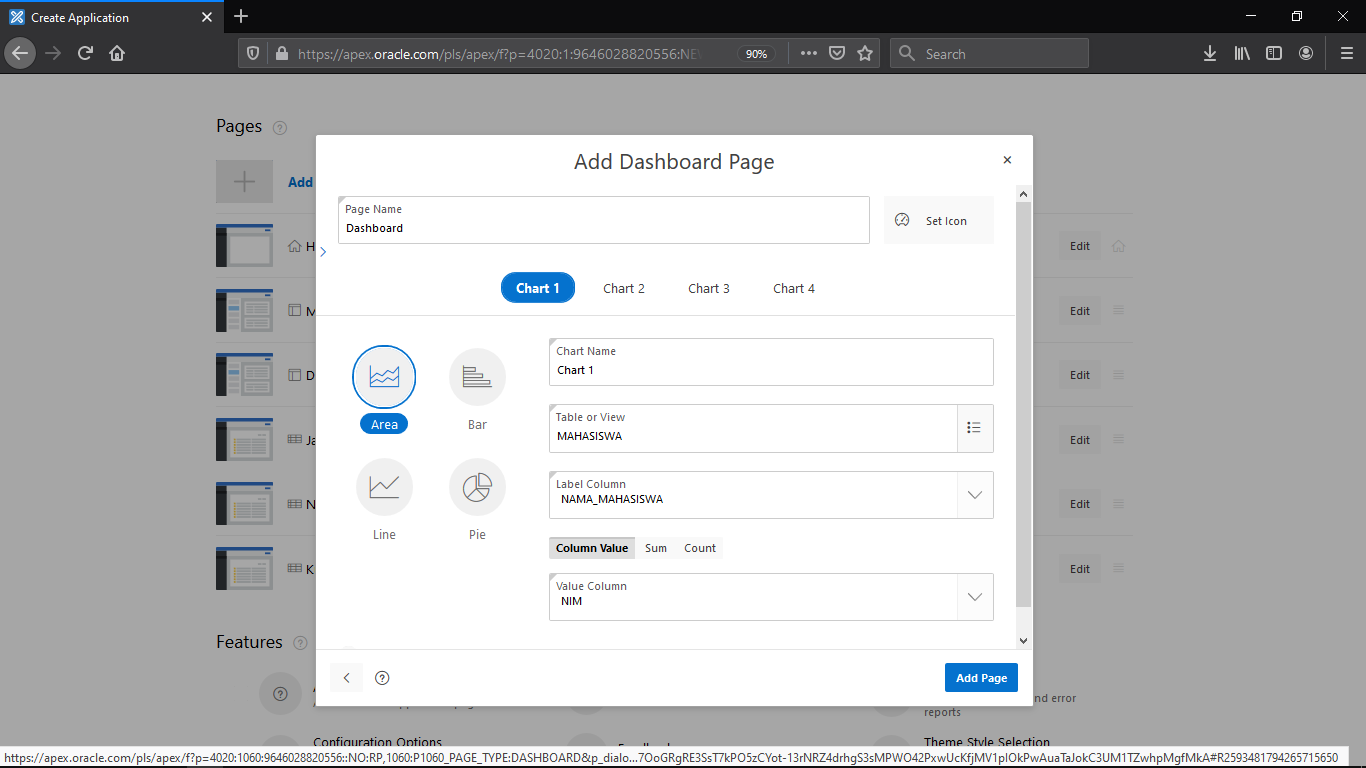
\includegraphics[scale=0.2]{figures/33.png}
    \caption{\textit{}}
        \end{center}
\label{gambar}
\end{figure}


\begin{figure}
\item[20].Dan juga di App Pagenya untuk Dosen, dan ikuti tampilan seperti dibawah ini.

    \begin{center}
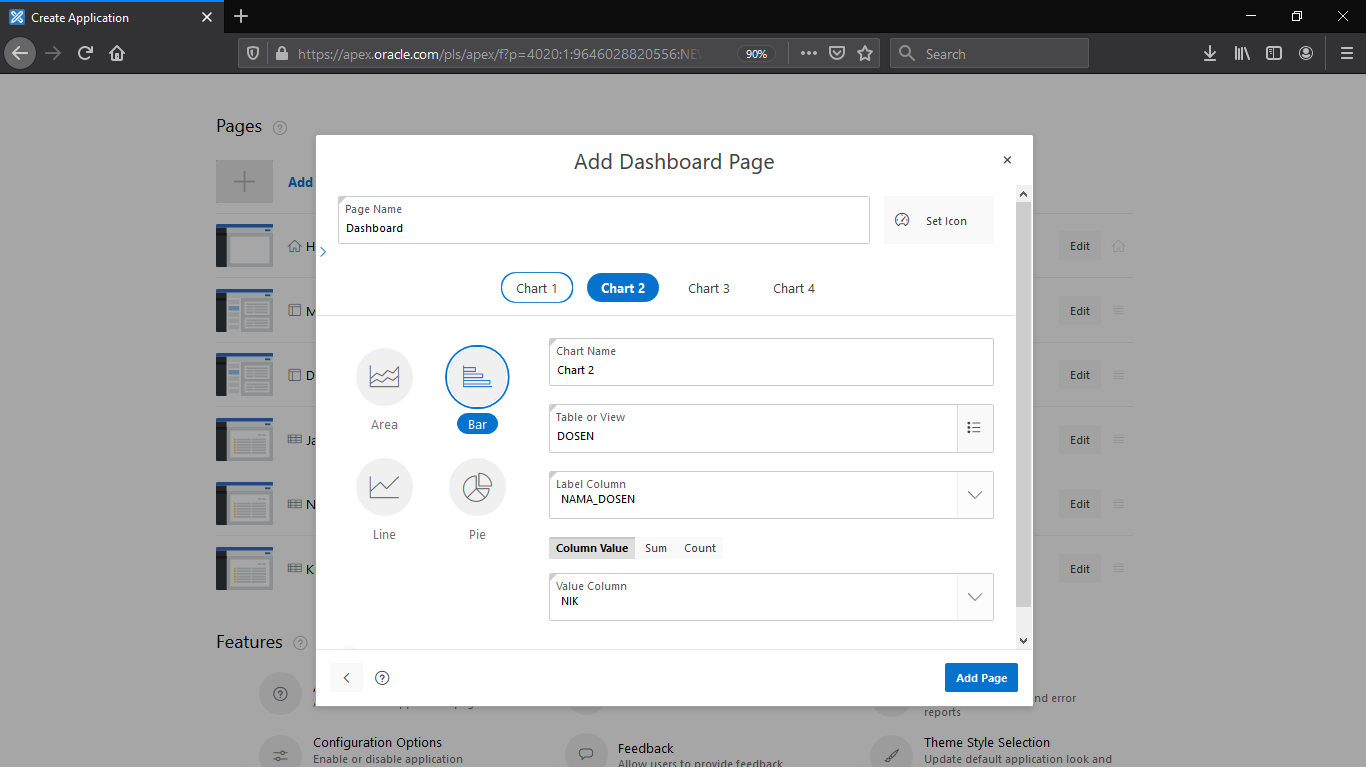
\includegraphics[scale=0.2]{figures/34.png}
    \caption{\textit{}}
        \end{center}
\label{gambar}
\end{figure}


\begin{figure}
\item[21]Dan juga di App Pagenya untuk Kuliah, dan ikuti tampilan seperti dibawah ini.

    \begin{center}
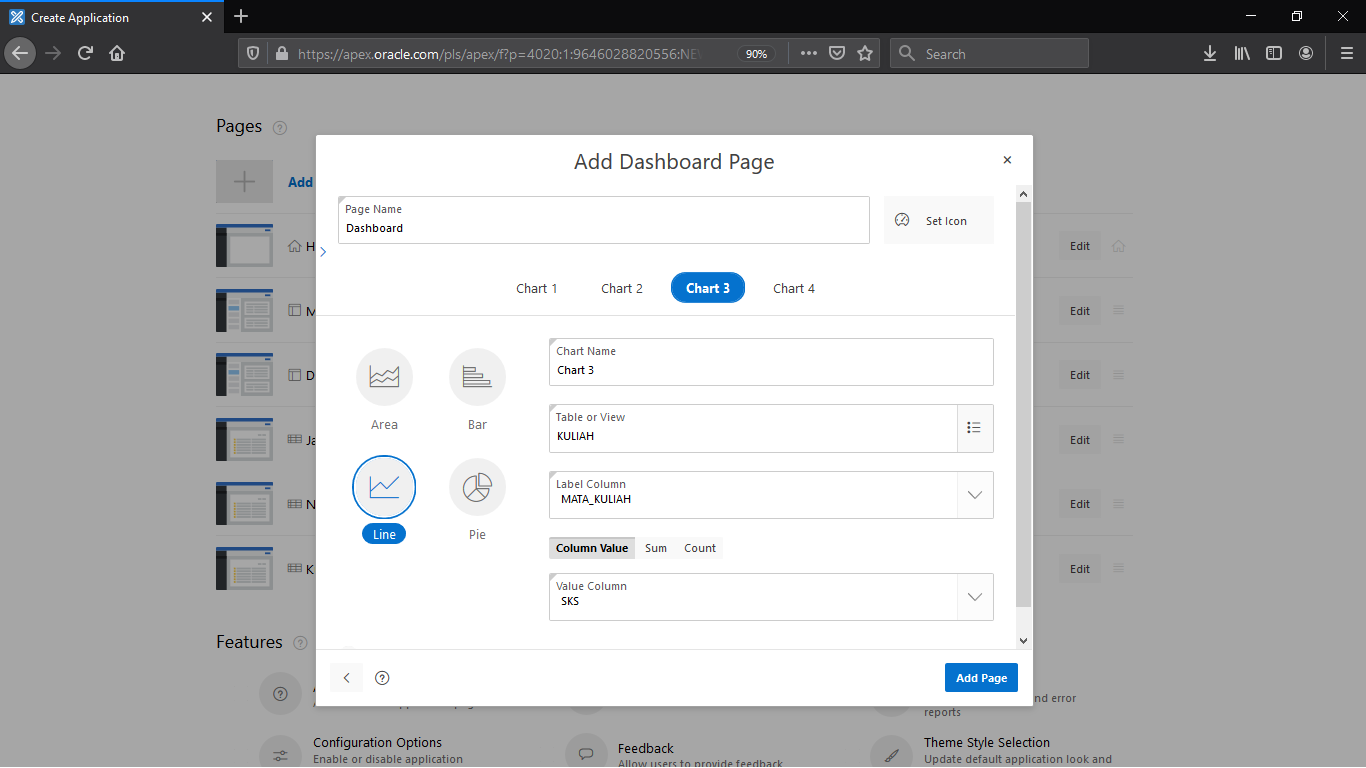
\includegraphics[scale=0.2]{figures/35.png}
    \caption{\textit{}}
        \end{center}
\label{gambar}
\end{figure}


\begin{figure}
\item[22]Dan juga di App Pagenya untuk Nilai, dan ikuti tampilan seperti dibawah ini.

    \begin{center}
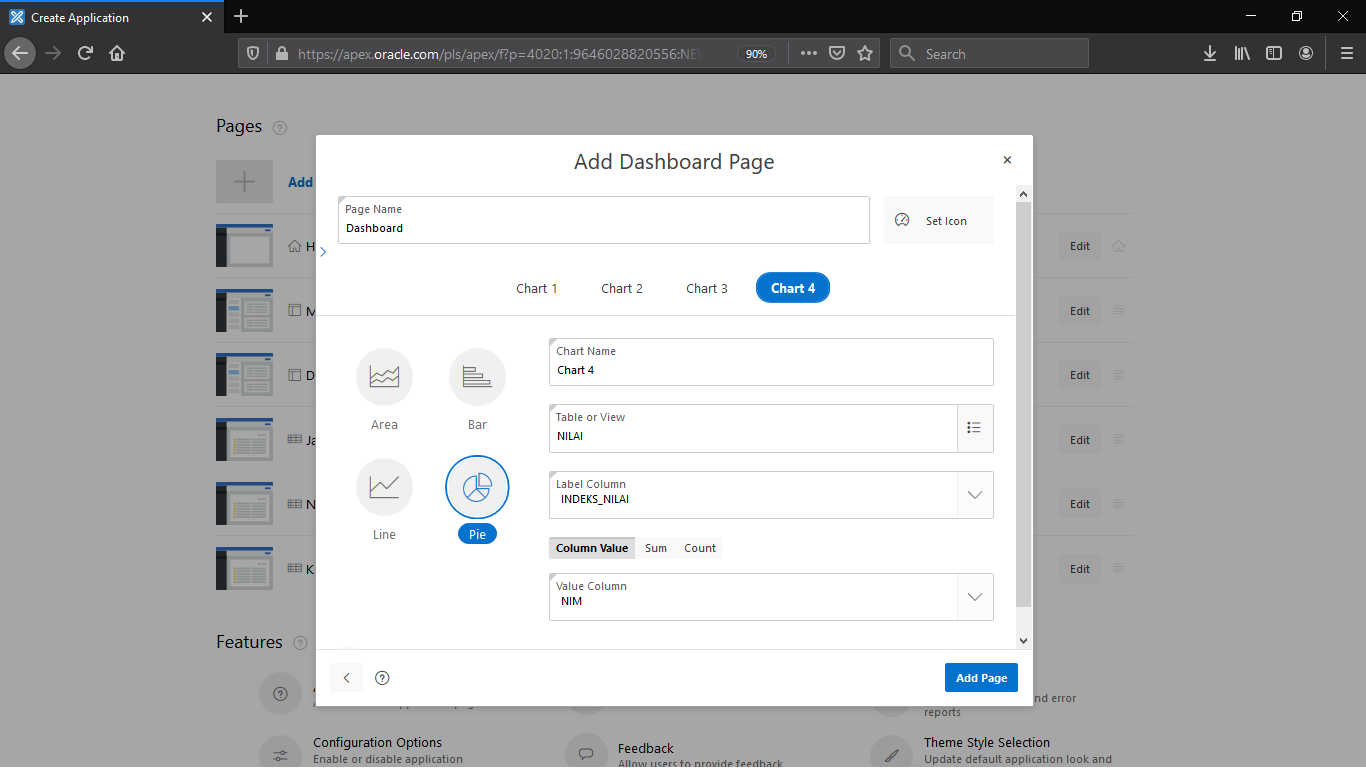
\includegraphics[scale=0.2]{figures/36.png}
    \caption{\textit{}}
        \end{center}
\label{gambar}
\end{figure}


\begin{figure}
\item[23]Dan Hasil Tampilan seperti ini jika sudah membuat Semua page.

    \begin{center}
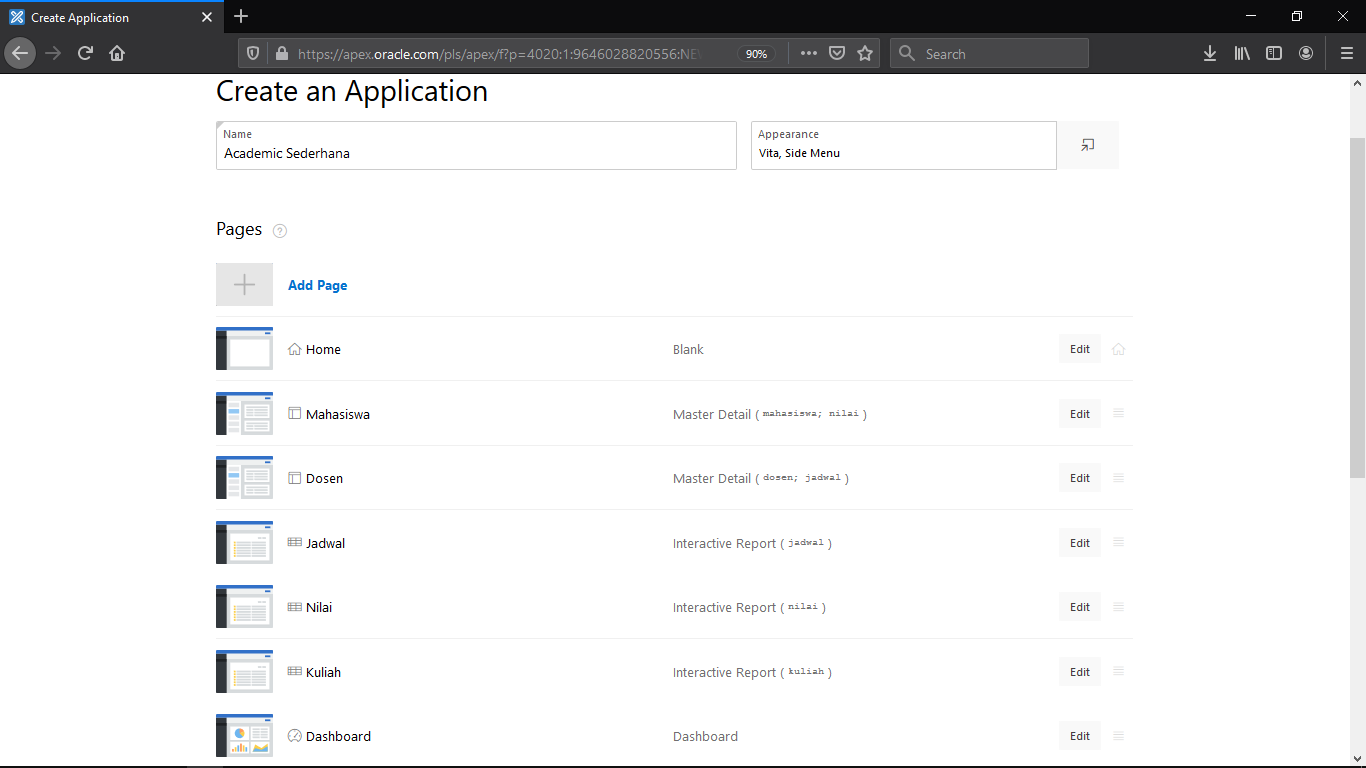
\includegraphics[scale=0.2]{figures/37.png}
    \caption{\textit{}}
        \end{center}
\label{gambar}
\end{figure}


\begin{figure}
\item[24]Lalu Scroll kebawah dan klik Check All pada Featuresnya setelah itu klik Create Application paling bawah, seperti tampilan dibawah ini.

    \begin{center}
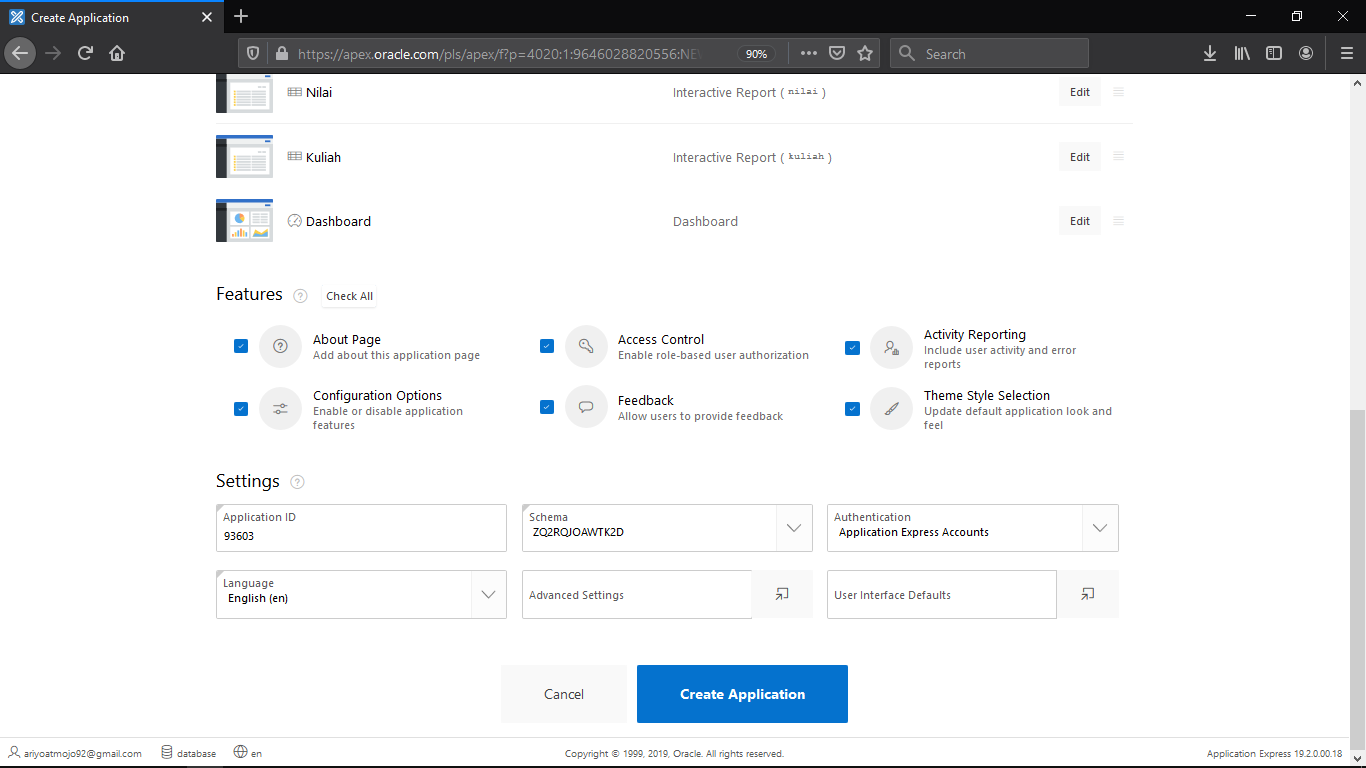
\includegraphics[scale=0.2]{figures/38.png}
    \caption{\textit{}}
        \end{center}
\label{gambar}
\end{figure}


\begin{figure}
\item[25]Setelah itu klik run Application.

    \begin{center}
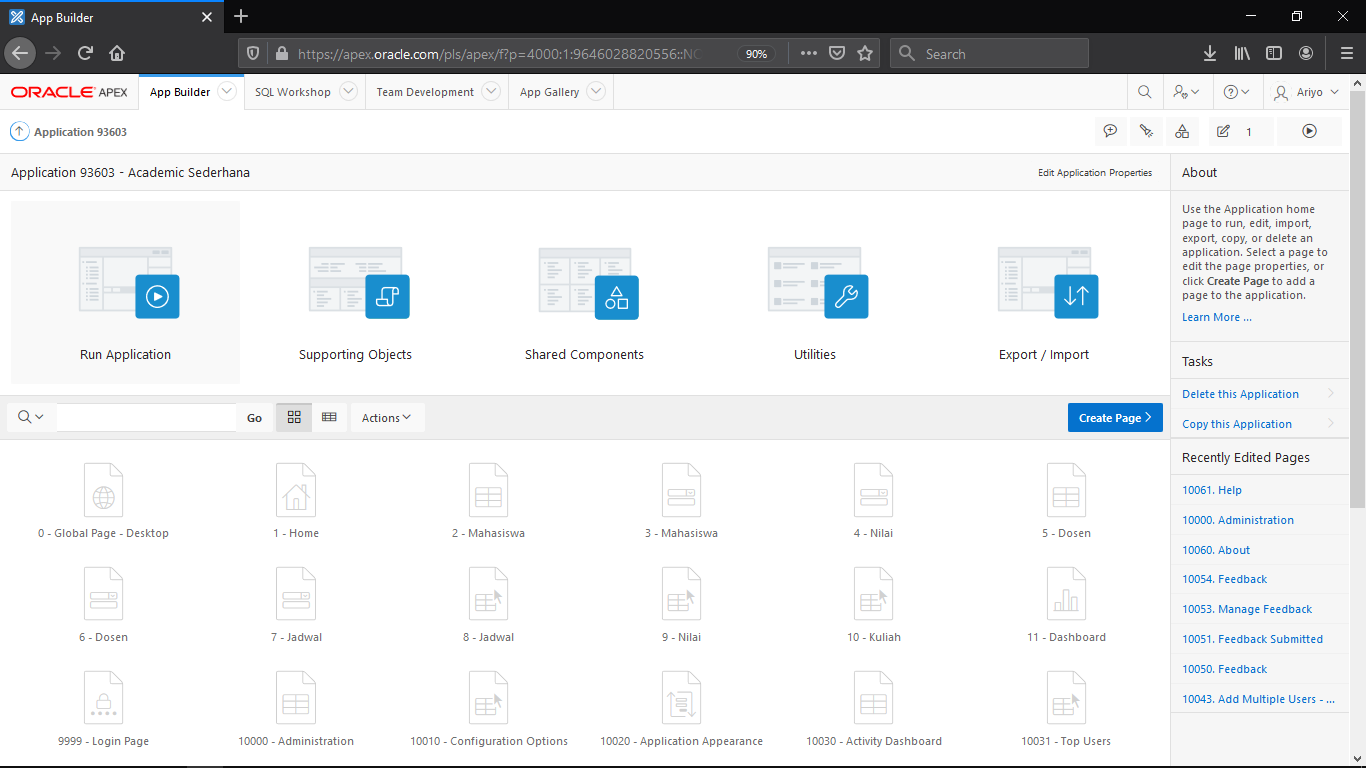
\includegraphics[scale=0.2]{figures/39.png}
    \caption{\textit{}}
        \end{center}
\label{gambar}
\end{figure}


\begin{figure}
\item[26]Dan tampilan hasil pembuatan aplikasi Academic Sederhana seperti dibawah ini.

    \begin{center}
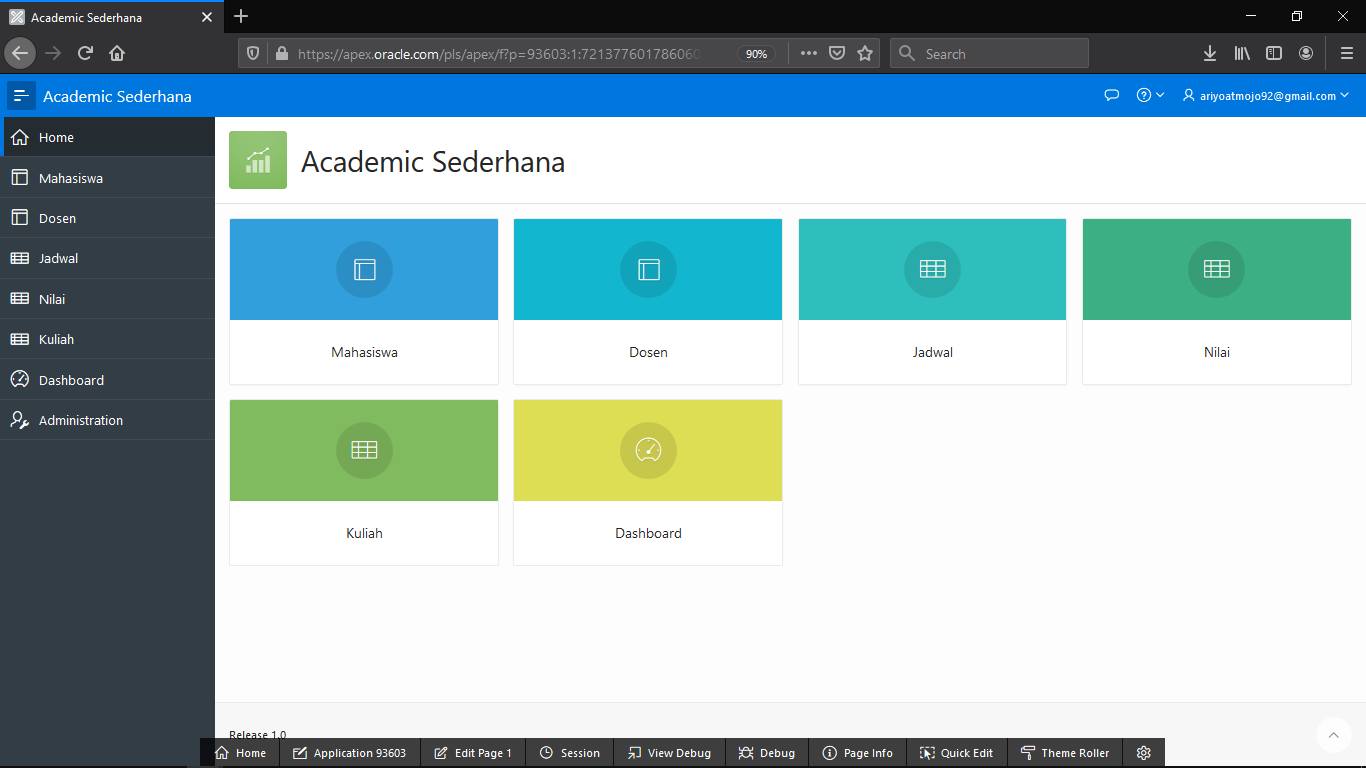
\includegraphics[scale=0.2]{figures/40.png}
    \caption{\textit{Tampilan Berhasil.}}
        \end{center}
\label{gambar}
\end{figure}


\begin{figure}
\item[27]Link login aplikasinya dibawah ini.
    \begin{center}
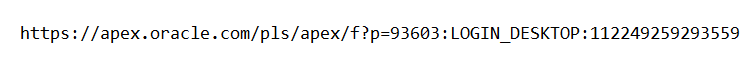
\includegraphics[scale=0.7]{figures/link.PNG}
    \caption{\textit{Tampilan Link.}}
        \end{center}
\item[28] username   : ariyoatmojo92@gmail.com
\item[29] kata sandi : playhard21, seperti digambar berikut
    \begin{center}
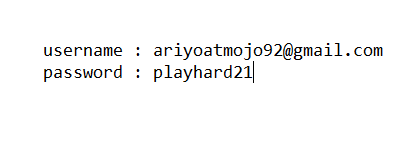
\includegraphics[scale=0.9]{figures/login.PNG}
    \caption{\textit{Username}}
        \end{center}
\label{gambar}
\end{figure}

\end{enumerate}
